\documentclass[conference]{IEEEtran}
\IEEEoverridecommandlockouts

\usepackage{cite}
\usepackage{amsmath,amssymb,amsfonts,amsthm}
\usepackage{algorithmic}
\usepackage{graphicx}
\usepackage{textcomp}
\usepackage{xcolor}
\usepackage{booktabs}
\usepackage{array}
\usepackage{url}
\usepackage{bm}
\usepackage{pgfplots}
\pgfplotsset{compat=1.18}

\newtheorem{theorem}{Theorem}
\newtheorem{definition}{Definition}
\newtheorem{proposition}{Proposition}
\newtheorem{remark}{Remark}

\def\BibTeX{{\rm B\kern-.05em{\sc i\kern-.025em b}\kern-.08em
    T\kern-.1667em\lower.7ex\hbox{E}\kern-.125emX}}

\begin{document}

\title{Catching the Wave Without Wiping Out: A Quantitative Risk Handbook for Retail Investors in the 2026 IPO Cycle}

\author{\IEEEauthorblockN{Surya Rao Rayarao}
\IEEEauthorblockA{\textit{Department of Statistics and Data Sciences} \\
\textit{Department of Computer Science} \\
\textit{The University of Texas at Austin}\\
Austin, TX, USA \\
suryarao.r@utexas.edu}
\and
\IEEEauthorblockN{Naga Donikena}
\IEEEauthorblockA{\textit{Department of Statistics and Data Sciences} \\
\textit{Department of Computer Science} \\
\textit{The University of Texas at Austin}\\
Austin, TX, USA \\
naga.donikena@utexas.edu}
}

\maketitle

\begin{abstract}
Public-market observers widely expect the next several months to bring a dense pipeline of initial public offerings (IPOs) spanning artificial-intelligence infrastructure, fintech, biotechnology, consumer-internet, and space and defense technology firms. Periods of this kind---``IPO windows'' or ``hot-issue markets''---reliably generate intense retail-investor interest, fueled by media coverage, first-day price spikes, and the fear of missing out on the next transformative company while it is still cheap. They also reliably generate a body of empirical finance research showing that the *statistical* profile of IPO investing is considerably less attractive to the ordinary investor than the headlines suggest: structurally asymmetric information, a documented long-run underperformance ``puzzle,'' lock-up-driven supply shocks, and return distributions with high variance and heavy right tails that reward a small number of outsized winners while a much larger number of issues disappoint. This paper assembles, in one place and at a level accessible to a non-specialist, the academic evidence on IPO risk and the mathematical machinery---Markowitz mean-variance optimization, the statistics of diversification, the Kelly criterion for position sizing, dollar-cost averaging, options-based hedging, and indexing---that a disciplined retail investor can use to participate in an IPO wave while bounding the downside. We work through fully specified numerical examples, present stylized illustrative charts that mirror the magnitude and direction of published empirical findings, and conclude with a step-by-step decision checklist and a worked case study comparing a concentrated ``hero bet'' strategy against a small, diversified satellite allocation layered on top of a low-cost index core. The throughline is simple and provable: the same enthusiasm that makes IPOs exciting also makes them dangerous in concentrated form, and basic, well-established quantitative discipline---not stock-picking skill---is what converts that excitement into a repeatable contribution to long-run wealth.
\end{abstract}

\begin{IEEEkeywords}
initial public offerings, IPO underpricing, retail investing, portfolio theory, diversification, Kelly criterion, risk management, behavioral finance, dollar-cost averaging, index investing
\end{IEEEkeywords}

% ============================================================
\section{Introduction}
\label{sec:intro}
% ============================================================

Equity markets move in cycles, and one of the most visible of these cycles is the rhythm of initial public offerings. When valuations are buoyant, financing is cheap, and investor sentiment is optimistic, the population of large private companies that have been ``waiting for the right window'' tends to file for listing in clusters \cite{lucasmcdonald1990}. Financial commentary in the months leading up to mid-2026 has pointed to exactly this kind of buildup: a substantial roster of large, well-known private technology, financial-technology, biotechnology, and infrastructure companies reportedly preparing registration statements, alongside a broader recovery in IPO issuance volumes after a multi-year lull. Whatever the precise roster of names that ultimately reaches the market---and that roster will continue to change as filings are confirmed, postponed, or withdrawn---the *structural* features of an active IPO window are well understood and remarkably stable across decades and geographies \cite{ritter1991, loughranritter2004}.

For a regular investor---someone investing primarily for retirement, a home purchase, a child's education, or simply long-run financial independence, rather than as a professional allocator with research staff and privileged deal access---an active IPO season presents a genuine opportunity wrapped in a genuine hazard. The opportunity is real: some IPOs go on to become generational compounders, and being an early shareholder in such a company is, in hindsight, one of the most lucrative things an investor can do. The hazard is equally real and considerably better documented: decades of empirical research show that the *population* of IPOs, taken as a whole, has historically (i) popped sharply on the first day of trading, (ii) been disproportionately allocated to institutional buyers rather than retail buyers in the most attractive deals (a phenomenon known as the ``winner's curse''), and (iii) underperformed comparable seasoned firms over the subsequent three to five years \cite{ibbotson1975, rock1986, loughranritter1995}. In other words, the public, retail-accessible slice of the IPO opportunity set is, on average, the slice with the least favorable risk-adjusted economics---precisely the slice that generates the most media excitement.

This paper's purpose is not to discourage participation in the coming IPO wave, nor to claim that no IPO is worth owning. It is to equip a regular investor with the same basic quantitative tools that professional risk managers use to convert an exciting-but-risky opportunity into a bounded, survivable, portfolio-level decision. None of the mathematics here is exotic or proprietary: mean-variance portfolio construction \cite{markowitz1952}, the statistics of diversification \cite{benartzithaler2001}, the Kelly criterion for bet sizing \cite{kelly1956}, the elementary algebra of dollar-cost averaging, and basic options-based hedges derived from the Black--Scholes framework \cite{blackscholes1973} have all been textbook material for fifty years or more \cite{bodiekanemarcus}. What is less common is seeing them assembled, with worked numbers, specifically around the IPO decision that a regular investor is likely to face several times over the coming months.

The remainder of this paper is organized as follows. Section~\ref{sec:background} reviews how an IPO actually works and why IPO activity arrives in waves. Section~\ref{sec:disadvantage} explains, with a short formal model, why retail investors face a structural information and allocation disadvantage in the IPO process (the winner's curse), and surveys the empirical evidence on first-day pops and long-run underperformance. Section~\ref{sec:risk} characterizes the statistical shape of IPO risk---volatility, skewness, and the lock-up cliff---using stylized illustrative charts calibrated to the magnitudes reported in the literature. Section~\ref{sec:strategies} is the heart of the handbook: it derives, with worked numerical examples, five complementary risk-reduction techniques---mean-variance allocation, the mathematics of diversification, fractional-Kelly position sizing, staggered entry (dollar-cost averaging), and index-fund ``capture'' of eventual winners. Section~\ref{sec:hedging} covers basic hedging instruments available to retail investors who do choose to hold individual IPO positions. Section~\ref{sec:case} assembles all of the above into a single worked case study contrasting a concentrated bet with a diversified satellite allocation. Section~\ref{sec:behavioral} reviews the behavioral biases that make IPO seasons particularly hazardous and how to pre-commit against them. Section~\ref{sec:checklist} distills everything into a one-page decision checklist for the months ahead, and Section~\ref{sec:conclusion} concludes.

\begin{remark}
\textbf{On the data used in this paper.} Several figures in this paper are explicitly labeled \emph{stylized illustrative data}. They are constructed to match the documented \emph{direction and rough magnitude} of findings in the peer-reviewed literature cited alongside them (e.g., the average first-day return, the average three-year underperformance gap, and typical post-listing volatility levels reported by Ritter, Loughran, and Ibbotson and updated periodically on Jay Ritter's IPO data repository). They are \emph{not} a forecast of the returns of any specific 2026 listing, and no statement in this paper should be read as investment advice regarding any named or unnamed company. Their purpose is solely to make the shape of the underlying statistical phenomena---skewness, long-run drift, variance decay under diversification---visually concrete for a non-specialist reader.
\end{remark}

% ============================================================
\section{Background: How IPOs Work and Why They Arrive in Waves}
\label{sec:background}
% ============================================================

\subsection{The Mechanics of Going Public}

An initial public offering converts a privately held company into a publicly traded one by selling newly issued (or existing-investor-owned) shares to outside investors for the first time. The standard U.S.-style process proceeds roughly as follows:

\begin{enumerate}
    \item \textbf{Engagement of underwriters.} The company hires one or more investment banks to manage the offering. The lead underwriter performs due diligence, helps draft the registration statement (the prospectus, e.g., Form S-1 in the United States), and assembles an underwriting syndicate.
    \item \textbf{Bookbuilding and roadshow.} The underwriters market the deal to large institutional investors---mutual funds, pension funds, hedge funds, and sovereign wealth funds---gauging demand at a range of prices. This process, called \emph{bookbuilding}, is the central mechanism by which the offer price is set \cite{rock1986}.
    \item \textbf{Pricing and allocation.} The night before trading begins, the underwriters and the company set a final offer price and decide how to allocate shares among the investors who indicated interest. Allocation decisions are at the underwriters' discretion and are well documented to favor large, repeat institutional clients \cite{ritter1991}.
    \item \textbf{First-day trading (the ``pop'').} Shares begin trading on an exchange. The difference between the first-day closing price and the offer price is the \emph{initial return} or ``pop,'' and is the statistic most widely reported in the financial press.
    \item \textbf{Lock-up expiration.} Pre-IPO shareholders---founders, employees, and venture investors---are typically restricted from selling for a fixed period, commonly 90--180 days. When the lock-up expires, a large supply of shares can become eligible for sale essentially overnight, frequently producing a measurable negative price effect known as the \emph{lock-up cliff} \cite{loughranritter2004}.
    \item \textbf{The ``greenshoe'' / over-allotment option.} Underwriters typically retain the right to sell up to an additional 15\% of the offering, which they use to stabilize the price in the days immediately following listing.
\end{enumerate}

Two features of this process matter enormously for a retail investor's risk exposure. First, the price that retail investors typically transact at is \emph{not} the IPO offer price---it is the price at which shares trade on the open market after institutions have already received their (often-profitable) allocations. Second, the supply of shares available to trade is itself a moving target: it expands sharply at the lock-up date, often before the company has reported more than one or two quarters of public financial results.

\subsection{Why IPO Activity Comes in Waves}

The clustering of IPO activity into discrete ``hot'' and ``cold'' windows has been studied extensively. Lucas and McDonald \cite{lucasmcdonald1990} model this as a rational response to asymmetric information: firms with favorable private information about their prospects prefer to issue equity when the market, on average, is more optimistic (and hence the cost of issuing mispriced equity is lower), producing clustering around periods of rising aggregate valuations. A complementary explanation is simply that going public is expensive and risky to attempt in a falling or volatile market---underwriters are reluctant to commit capital, and investor demand for new, unproven names contracts sharply during downturns. The result, empirically, is that IPO volume tracks the broad equity cycle with a lag: a sustained rally in public-market valuations is reliably followed, some quarters later, by a surge in new listings, as companies that delayed their IPO during the prior downturn move to capture favorable pricing \cite{loughranritter2004}.

This dynamic is directly relevant to how a regular investor should interpret an active IPO season. A wave of IPOs is, almost definitionally, a symptom of an environment in which (a) public-market valuations have already risen substantially, (b) issuers and their bankers believe current prices are favorable \emph{to the seller}, and (c) a large number of new, statistically unproven names will compete for investor attention and capital simultaneously. None of this means the broad market is overvalued, nor that any particular company is a poor investment---but it does mean that the population-level base rates discussed in Section~\ref{sec:disadvantage} are the ones a regular investor should expect to face, on average, across the dozens of new names that will be marketed to them over the coming months.

\subsection{The Anticipated 2026 Pipeline, in General Terms}

Rather than naming specific companies whose filing status, pricing, and timing remain fluid (and may have changed by the time this paper is read), we characterize the anticipated pipeline by \emph{category}, which is the level at which a regular investor's planning should occur in any case:

\begin{itemize}
    \item \textbf{AI infrastructure and compute.} Firms supplying chips, cloud capacity, data-center hardware, and foundation-model platforms have been widely reported as leading candidates, reflecting the broader AI investment cycle.
    \item \textbf{Fintech and digital payments.} Several large, well-funded private payment, lending, and ``neobank'' platforms have reportedly explored listings as funding markets normalized.
    \item \textbf{Biotechnology and health technology.} Clinical-stage and platform biotech firms typically make up a large share of any active issuance window, and are characterized by binary, trial-readout-driven risk profiles distinct from the technology names that dominate headlines.
    \item \textbf{Consumer internet, creator economy, and gaming.} Consumer-facing platforms with large user bases but sometimes-unproven monetization models recur in every IPO cycle.
    \item \textbf{Space, defense, and advanced industrials.} A smaller but growing category reflecting renewed public and private investment in these sectors.
\end{itemize}

The remainder of this paper applies equally to all of these categories: the structural features of the IPO process (Section~\ref{sec:background}), the statistical disadvantages facing retail buyers (Section~\ref{sec:disadvantage}), and the risk-reduction toolkit (Sections~\ref{sec:risk}--\ref{sec:hedging}) do not depend on the specific sector, and a prudent investor should apply the same discipline to an AI-infrastructure listing as to a biotech or consumer-internet one.

% ============================================================
\section{Why the Odds Are Structurally Tilted Against the Retail Buyer}
\label{sec:disadvantage}
% ============================================================

\subsection{The Winner's Curse: A Short Formal Model}

Kevin Rock's classic model \cite{rock1986} explains a puzzle that, at first glance, seems backwards: if IPOs are, on average, underpriced (i.e., they tend to pop on the first day), why doesn't every investor simply buy every IPO at the offer price and collect the average pop? The answer is that \emph{not every investor can get an allocation in every deal}, and the deals they are most likely to be \emph{rationed out of} are precisely the ones that turn out to be the most underpriced (because informed institutional investors crowd in to claim shares of the good deals and stay away from the bad ones).

Formally, suppose there are two types of IPOs: ``good'' deals with expected initial return $r_G > 0$ and ``bad'' deals with expected initial return $r_B < 0$ (i.e., they tend to be \emph{overpriced} relative to fair value and underperform immediately). Let $p$ be the (unconditional) probability that any given IPO is a ``good'' deal. Informed investors (large institutions with research capacity and underwriter relationships) can distinguish good deals from bad ones and apply for shares only in good deals; uninformed investors (most retail participants) cannot distinguish them and apply for shares in every deal.

When demand for an oversubscribed ``good'' deal exceeds supply, the underwriter rations shares pro rata across all applicants---informed and uninformed alike. When a ``bad'' deal is undersubscribed (because informed investors avoid it), uninformed investors receive their \emph{full} requested allocation. Consequently, the uninformed investor's allocation-weighted expected return is
\begin{equation}
E[r \mid \text{uninformed}] = \frac{\alpha\, p\, r_G + (1-p)\, r_B}{\alpha\, p + (1-p)},
\label{eq:winners-curse}
\end{equation}
where $\alpha \in (0,1]$ is the fraction of a ``good'' deal's shares that remains for uninformed investors after informed investors are served (with $\alpha < 1$ because the deal is oversubscribed). Because $\alpha < 1$ shrinks the weight on the favorable outcome $r_G$ relative to its true population frequency $p$, while the unfavorable outcome $r_B$ retains its full weight $(1-p)$, we have
\begin{equation}
E[r \mid \text{uninformed}] \;<\; E[r] = p\, r_G + (1-p)\, r_B.
\end{equation}
This is the \emph{winner's curse}: conditioning on actually \emph{receiving} an allocation is itself bad news, because allocations are easiest to obtain precisely in the deals that are least attractive. Rock shows that, in equilibrium, issuers must underprice IPOs \emph{on average} (i.e., set $E[r] > 0$) simply to keep uninformed investors willing to participate at all---the average pop reported breathlessly in the press is, in a real sense, the minimum bribe required to keep retail money in the game, not a reflection of the return retail investors can actually expect to realize across a portfolio of deals.

\begin{remark}
A regular investor who reads ``the average IPO pops 20\% on day one'' should not infer that they can expect to capture anything close to 20\% by buying IPOs. They should infer the opposite: in any deal where they can easily get shares at the offer price, they are statistically more likely to be holding a below-average deal, and in any deal that is so popular they cannot get an allocation at the offer price, they will be buying at the already-elevated opening trade price---at which point the ``pop'' has already accrued to someone else.
\end{remark}

\subsection{Empirical Evidence: First-Day Pops and the Long-Run Underperformance Puzzle}

The phenomenon described abstractly above shows up cleanly in the data. Ibbotson's foundational study \cite{ibbotson1975} and Ritter's subsequent large-sample analyses \cite{ritter1991} documented average U.S. first-day initial returns in the high single digits to high teens (with substantial variation across hot and cold markets, occasionally spiking far higher during speculative episodes). At the same time, Ritter \cite{ritter1991} and, more comprehensively, Loughran and Ritter \cite{loughranritter1995} documented that firms going public substantially \emph{underperform} a matched sample of seasoned, comparable firms over the subsequent three to five years---the so-called ``new issues puzzle.'' Figure~\ref{fig:popdist} and Figure~\ref{fig:longrun} render these two stylized facts visually.

\begin{figure}[!t]
\centering
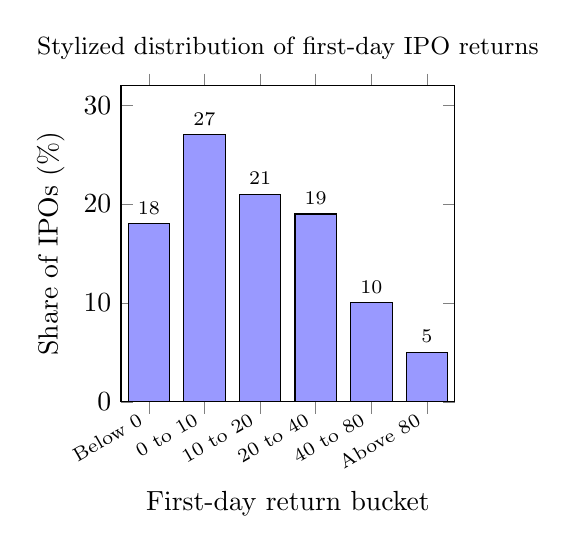
\begin{tikzpicture}
\begin{axis}[
    ybar,
    bar width=15pt,
    xlabel={First-day return bucket},
    ylabel={Share of IPOs (\%)},
    symbolic x coords={Below 0,0 to 10,10 to 20,20 to 40,40 to 80,Above 80},
    xtick=data,
    x tick label style={font=\scriptsize, rotate=30, anchor=east},
    ymin=0, ymax=32,
    width=0.48\textwidth, height=5.6cm,
    nodes near coords,
    every node near coord/.append style={font=\scriptsize},
    title={\small Stylized distribution of first-day IPO returns}
]
\addplot[fill=blue!40] coordinates {(Below 0,18) (0 to 10,27) (10 to 20,21) (20 to 40,19) (40 to 80,10) (Above 80,5)};
\end{axis}
\end{tikzpicture}
\caption{Stylized illustrative distribution of first-day IPO returns, shaped to match the well-documented qualitative pattern: a meaningful fraction of deals (roughly one in six to one in five, historically) open \emph{below} the offer price, the bulk cluster in single- to low-double-digit gains, and a long right tail of large ``pops'' accounts for a small share of deals but a disproportionate share of the headlines \cite{ibbotson1975,ritter1991}. The right-skew is the key feature: the \emph{average} pop is pulled upward by a minority of spectacular outcomes, while the \emph{median} and \emph{modal} outcomes are far more modest---and a non-trivial share of deals lose money immediately.}
\label{fig:popdist}
\end{figure}

\begin{figure}[!t]
\centering
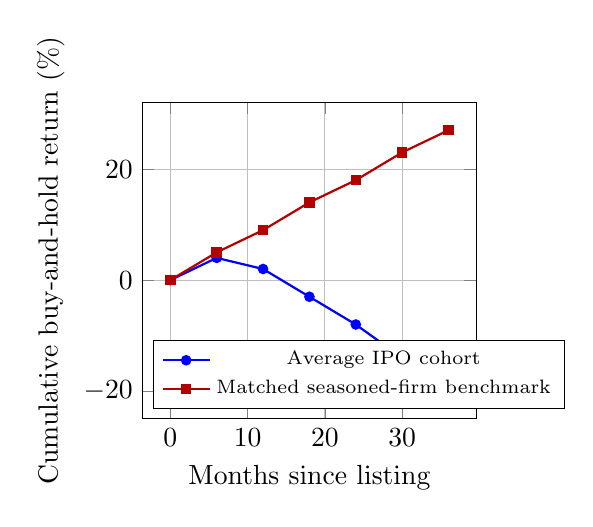
\begin{tikzpicture}
\begin{axis}[
    xlabel={Months since listing},
    ylabel={Cumulative buy-and-hold return (\%)},
    legend pos=south west,
    legend style={font=\scriptsize},
    width=0.48\textwidth, height=5.6cm,
    grid=both,
    ymin=-25, ymax=32
]
\addplot[blue, thick, mark=*, mark size=1.5pt] coordinates {(0,0)(6,4)(12,2)(18,-3)(24,-8)(30,-14)(36,-20)};
\addlegendentry{Average IPO cohort}
\addplot[red!70!black, thick, mark=square*, mark size=1.5pt] coordinates {(0,0)(6,5)(12,9)(18,14)(24,18)(30,23)(36,27)};
\addlegendentry{Matched seasoned-firm benchmark}
\end{axis}
\end{tikzpicture}
\caption{Stylized illustration of the ``new issues puzzle'' documented by Loughran and Ritter \cite{loughranritter1995} and Ritter \cite{ritter1991}: a cohort of newly listed firms, tracked from their first trading day, has historically underperformed a benchmark of comparable seasoned firms by a wide and widening margin over a three-year horizon, even though the same cohort, on average, opened at a premium to its offer price. The crossing of the two curves around month 12--18 is the empirical heart of the puzzle---the very feature that makes IPOs look most attractive (the early pop) is statistically uninformative about, and in aggregate inversely related to, their multi-year performance.}
\label{fig:longrun}
\end{figure}

Two clarifications are essential. First, these are \emph{population averages}: any individual IPO can and frequently does defy the pattern, and a number of the most consequential companies of the last several decades were, in fact, IPOs that went on to vastly outperform. Second, the underperformance documented by Loughran and Ritter is concentrated disproportionately in certain sub-populations---younger, smaller, more speculative, and more ``story-driven'' firms tend to show the largest gap, while larger, more established issuers with longer operating histories show a much smaller (and in some sub-samples, statistically indistinguishable from zero) gap \cite{loughranritter2004}. This sub-population heterogeneity is itself useful information: it suggests that \emph{which kind} of IPO an investor leans toward is at least as important as \emph{whether} they participate at all---a theme we return to in Section~\ref{sec:strategies}.

\subsection{The Retail Trading Penalty}

A separate and complementary line of research, exemplified by Barber and Odean \cite{barberodean2000}, finds that individual investors who trade actively---buying into hot names, selling losers, chasing recent performance---underperform the market and underperform their own buy-and-hold counterfactual by a wide margin, with the gap attributable in large part to transaction costs and to systematically poor timing of entries and exits. IPO investing, by its nature, is a high-attention, high-emotion, high-frequency-of-decision activity (when does the lock-up expire? should I buy the dip after the pop fades? should I average down?), and is therefore precisely the kind of activity in which the Barber--Odean ``trading is hazardous to your wealth'' effect is likely to compound the population-level IPO effects discussed above. The risk-reduction techniques in Section~\ref{sec:strategies} are designed, in part, specifically to minimize the number and frequency of \emph{ad hoc} trading decisions an investor must make.

% ============================================================
\section{The Statistical Shape of IPO Risk}
\label{sec:risk}
% ============================================================

\subsection{Volatility and Beta Instability}

Newly listed firms typically exhibit (i) higher return volatility than seasoned firms of comparable size and sector, (ii) unstable estimated market betas during the first several quarters of trading (because there is too little price history to estimate beta reliably, and because the firm's true risk profile may still be evolving rapidly), and (iii) elevated idiosyncratic (i.e., diversifiable, firm-specific) variance relative to systematic (market-wide) variance. This last point is the one that matters most for portfolio construction: idiosyncratic variance is, by definition, the kind of risk that diversification can remove without sacrificing expected return, whereas systematic variance cannot be diversified away. A newly listed stock is, in a meaningful statistical sense, \emph{mostly idiosyncratic risk}---which is exactly the kind of risk a regular investor should not want to hold in concentrated form (Section~\ref{sec:mpt}).

\subsection{The Lock-Up Cliff as a Predictable Supply Shock}

The lock-up expiration described in Section~\ref{sec:background} deserves special quantitative attention because, unlike most sources of stock-price risk, its \emph{timing} is public information disclosed in the prospectus. Event-study methodology---a standard tool in empirical finance---measures the \emph{cumulative abnormal return} (CAR) around an event date $\tau$ as
\begin{equation}
\text{CAR}(\tau_1, \tau_2) = \sum_{t=\tau_1}^{\tau_2} \big( R_{i,t} - E[R_{i,t} \mid \mathcal{F}_{t-1}] \big),
\label{eq:car}
\end{equation}
where $R_{i,t}$ is firm $i$'s realized return on day $t$ and $E[R_{i,t} \mid \mathcal{F}_{t-1}]$ is its expected return conditional on information available the prior day (commonly estimated via a market or factor model). Studies applying this methodology around lock-up expiration dates have documented economically meaningful negative average abnormal returns in the days surrounding the event---consistent with a textbook supply-and-demand interpretation: a large, mechanically scheduled increase in the float of tradeable shares, often arriving before the company has built a long public track record, tends to depress the price, on average, holding all else equal \cite{loughranritter2004}.

\begin{remark}
The practical implication is not ``never buy near a lock-up date'' (timing markets around single, well-telegraphed events is itself a form of speculation, and the average effect, while real, is neither universal nor enormous at the individual-stock level). The practical implication is that an investor who is already holding a freshly listed stock should \emph{expect}, and size their position to be able to tolerate, a bout of elevated volatility and downward pressure around the lock-up date---and should not interpret such a move, in isolation, as new information about the company's fundamentals.
\end{remark}

\subsection{Putting It Together: Why a Single IPO Is a High-Variance, Right-Skewed Lottery Ticket}

Combining the observations above---high idiosyncratic volatility, unstable beta, a right-skewed (occasionally spectacular, more often disappointing) return distribution, and a scheduled negative-supply-shock event in the first several months of trading---the statistical profile of an individual, freshly purchased IPO share resembles what behavioral finance researchers call a \emph{lottery-like asset}: low probability of an extreme positive outcome, higher probability of a mediocre-to-negative outcome, and overall variance far higher than a diversified equity portfolio. None of this means an IPO cannot be a good investment for a particular investor in a particular amount; it means that the \emph{amount}---the position size relative to the rest of the portfolio---is the single most important decision the investor will make, and is the focus of the next section.

% ============================================================
\section{Five Mathematically Grounded Risk-Reduction Strategies}
\label{sec:strategies}
% ============================================================

This section is the practical core of the handbook. Each subsection derives a specific, well-established quantitative technique, applies it explicitly to the IPO decision, and works through fully specified numerical examples that a regular investor can replicate with a spreadsheet.

\subsection{Mean--Variance Allocation: Treat the IPO as a Satellite, Not the Core}
\label{sec:mpt}

Harry Markowitz's mean-variance framework \cite{markowitz1952} remains the standard starting point for thinking about how a risky new asset should be incorporated into an existing portfolio. Consider a portfolio that allocates a weight $w$ to a candidate IPO position (or a small basket of them) and weight $(1-w)$ to a diversified core (e.g., a low-cost total-market index fund). If the core has expected return $\mu_c$ and volatility $\sigma_c$, the IPO sleeve has expected return $\mu_s$ and volatility $\sigma_s$, and the correlation between the two is $\rho$, then the combined portfolio has
\begin{align}
E[R_p] &= w\,\mu_s + (1-w)\,\mu_c, \label{eq:mvret}\\
\sigma_p^2 &= w^2 \sigma_s^2 + (1-w)^2 \sigma_c^2 + 2 w (1-w) \rho\, \sigma_s \sigma_c. \label{eq:mvvar}
\end{align}

\begin{proposition}[Small allocations to high-variance, low-correlation assets can be efficient]
\label{prop:satellite}
Suppose $\sigma_s \gg \sigma_c$ (the IPO sleeve is much more volatile than the core) and $\rho$ is small or modestly positive (newly listed firms' idiosyncratic risk is, almost by construction, weakly correlated with the broad market in the short run). Then the marginal effect of a small increase in $w$ from zero on portfolio variance is approximately linear and bounded,
\[
\left.\frac{\partial \sigma_p^2}{\partial w}\right|_{w=0} = 2\big(\rho\,\sigma_s\sigma_c - \sigma_c^2\big),
\]
while the marginal effect on expected return is constant at $(\mu_s - \mu_c)$. Consequently, for sufficiently small $w$, the change in portfolio variance is second-order (proportional to $w^2 \sigma_s^2$ for the dominant term) while the change in expected return is first-order (proportional to $w$), so a small allocation can raise expected return materially while raising portfolio risk only marginally---\emph{provided} $w$ is kept small enough that the $w^2 \sigma_s^2$ term remains negligible relative to $\sigma_c^2$.
\end{proposition}

\noindent\textit{Worked example.} Let the core index have $\mu_c = 8\%$ and $\sigma_c = 16\%$ (broadly representative long-run U.S. equity figures), and let a basket of IPO satellite positions have $\mu_s = 12\%$ (a deliberately optimistic input, granting the satellite sleeve credit for the possibility of a long-run winner) and $\sigma_s = 45\%$ (consistent with the elevated volatility discussed in Section~\ref{sec:risk}), with $\rho = 0.3$. Table~\ref{tab:mvex} shows $E[R_p]$ and $\sigma_p$ for several allocation weights $w$.

\begin{table}[!t]
\centering
\caption{Mean--variance arithmetic for a core-plus-satellite portfolio (Eqs.~\ref{eq:mvret}--\ref{eq:mvvar}), $\mu_c=8\%$, $\sigma_c=16\%$, $\mu_s=12\%$, $\sigma_s=45\%$, $\rho=0.3$.}
\label{tab:mvex}
\begin{tabular}{@{}cccc@{}}
\toprule
Satellite weight $w$ & $E[R_p]$ & $\sigma_p$ & $E[R_p]/\sigma_p$ \\
\midrule
0\%   & 8.00\% & 16.00\% & 0.500 \\
5\%   & 8.20\% & 16.84\% & 0.487 \\
10\%  & 8.40\% & 18.05\% & 0.465 \\
20\%  & 8.80\% & 21.51\% & 0.409 \\
50\%  & 10.00\% & 33.04\% & 0.303 \\
100\% & 12.00\% & 45.00\% & 0.267 \\
\bottomrule
\end{tabular}
\end{table}

The arithmetic in Table~\ref{tab:mvex} makes the intuition concrete: moving from a 0\% to a 5\% satellite allocation raises expected return by 0.20 percentage points while raising volatility by only 0.84 percentage points---a very favorable trade. Moving from 50\% to 100\%, by contrast, raises expected return by only 2.0 percentage points while raising volatility by nearly 12 percentage points---an increasingly unfavorable trade, and one that drags the portfolio's reward-to-risk ratio (the simple ratio $E[R_p]/\sigma_p$, a close cousin of the Sharpe ratio \cite{sharpe1964}) sharply downward. Figure~\ref{fig:frontier} shows the same idea in efficient-frontier form: a small, deliberate satellite allocation can shift an investor's achievable risk-return menu modestly to the upper-left (more return per unit of risk), while a large allocation pushes the realized portfolio far out along a much steeper, less efficient segment of the curve.

\begin{figure}[!t]
\centering
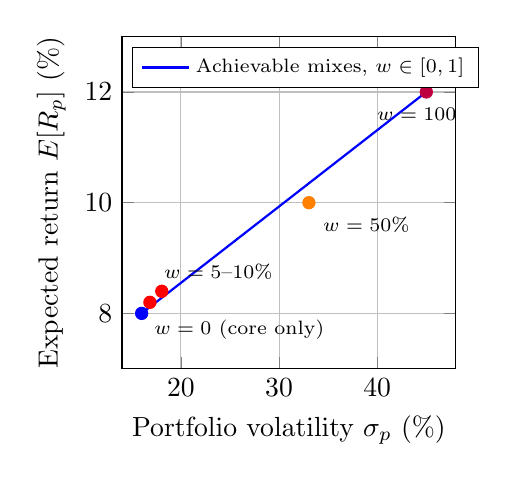
\begin{tikzpicture}
\begin{axis}[
    xlabel={Portfolio volatility $\sigma_p$ (\%)},
    ylabel={Expected return $E[R_p]$ (\%)},
    width=0.48\textwidth, height=5.8cm,
    legend pos=north west,
    legend style={font=\scriptsize},
    grid=both,
    xmin=14, xmax=48, ymin=7, ymax=13
]
\addplot[blue, thick, domain=16:45, samples=2] coordinates {(16,8) (45,12)};
\addlegendentry{Achievable mixes, $w \in [0,1]$}
\addplot[mark=*, only marks, mark size=2.2pt, blue] coordinates {(16,8)};
\addplot[mark=*, only marks, mark size=2.2pt, red] coordinates {(16.84,8.20)};
\addplot[mark=*, only marks, mark size=2.2pt, red] coordinates {(18.05,8.40)};
\addplot[mark=*, only marks, mark size=2.2pt, orange] coordinates {(33.04,10.00)};
\addplot[mark=*, only marks, mark size=2.2pt, purple] coordinates {(45,12)};
\node[anchor=west, font=\scriptsize] at (axis cs:16.3,7.7) {$w=0$ (core only)};
\node[anchor=west, font=\scriptsize] at (axis cs:17.3,8.75) {$w=5$--$10\%$};
\node[anchor=west, font=\scriptsize] at (axis cs:33.5,9.6) {$w=50\%$};
\node[anchor=west, font=\scriptsize] at (axis cs:39,11.6) {$w=100\%$};
\end{axis}
\end{tikzpicture}
\caption{The set of achievable risk-return combinations from mixing a diversified core ($\mu_c=8\%,\sigma_c=16\%$) with an IPO satellite sleeve ($\mu_s=12\%,\sigma_s=45\%,\rho=0.3$), per Table~\ref{tab:mvex}. Small satellite weights ($w=5$--$10\%$) buy a modest expected-return increase at a small risk cost and remain close to the efficient, low-volatility end of the curve; large weights buy a larger expected-return increase at a steeply disproportionate risk cost, and push the portfolio out toward the volatility profile of the satellite sleeve itself.}
\label{fig:frontier}
\end{figure}

\subsection{The Mathematics of Diversification: Why Eight Small Bets Beat One Big One}

A separate, complementary question is: \emph{given} that an investor has decided to devote some fixed fraction of their portfolio to IPO exposure, should they put it all into one name, or spread it across several? The relevant mathematics is the classical formula for the variance of an equally weighted portfolio of $N$ assets, each with variance $\sigma^2$ and pairwise correlation $\rho$ (assumed, for simplicity, equal across all pairs):
\begin{equation}
\sigma_N^2 = \frac{\sigma^2}{N} + \frac{N-1}{N}\,\rho\,\sigma^2 \;\xrightarrow{N \to \infty}\; \rho\,\sigma^2.
\label{eq:diversification}
\end{equation}
This identity---sometimes called the ``diversification decomposition''---is one of the most important results in all of portfolio theory, and it long predates, and underlies, the modern enthusiasm for ``naive'' $1/N$ diversification rules that have been shown to perform surprisingly well in practice \cite{benartzithaler2001}. It says that the variance of an equally weighted basket splits cleanly into two pieces: a \emph{diversifiable} piece, $\sigma^2/N$, that shrinks toward zero as the number of (imperfectly correlated) holdings grows, and a \emph{non-diversifiable} floor, $\frac{N-1}{N}\rho\sigma^2 \to \rho\sigma^2$, set entirely by the average pairwise correlation, that no amount of further diversification within the basket can remove.

\noindent\textit{Worked example.} Take $\sigma = 45\%$ (single-IPO annualized volatility, as in Section~\ref{sec:mpt}) and a modest average pairwise correlation of $\rho = 0.15$ (newly listed firms across different sectors and vintages are not strongly correlated with one another in the short run, though they share some common exposure to the broad ``risk-on/risk-off'' cycle that drives IPO sentiment generally). Equation~\eqref{eq:diversification} gives the basket volatility $\sigma_N = \sqrt{\sigma_N^2}$ shown in Figure~\ref{fig:diversification} for $N = 1, \dots, 30$.

\begin{figure}[!t]
\centering
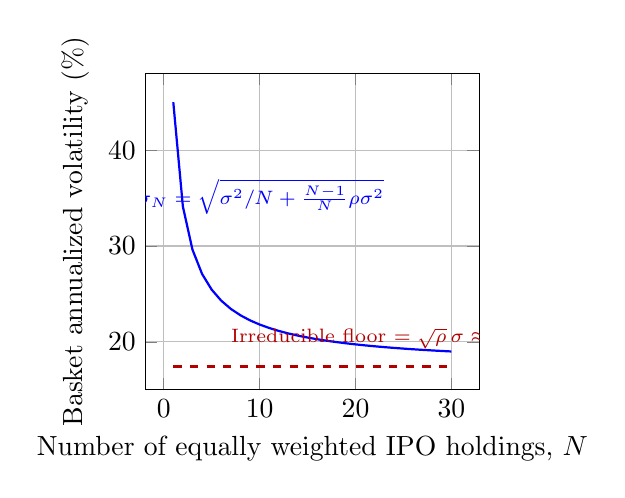
\begin{tikzpicture}
\begin{axis}[
    xlabel={Number of equally weighted IPO holdings, $N$},
    ylabel={Basket annualized volatility (\%)},
    width=0.48\textwidth, height=5.6cm,
    grid=both,
    ymin=15, ymax=48,
    domain=1:30, samples=30
]
\addplot[thick, blue] {sqrt( (45*45)/x + ((x-1)/x)*0.15*45*45 )};
\addplot[dashed, thick, red!70!black, domain=1:30, samples=2] coordinates {(1,17.43)(30,17.43)};
\node[anchor=south west, font=\scriptsize, red!70!black] at (axis cs:6,18.3) {Irreducible floor $=\sqrt{\rho}\,\sigma \approx 17.4\%$};
\node[anchor=north east, font=\scriptsize, blue] at (axis cs:24,38) {$\sigma_N=\sqrt{\sigma^2/N+\frac{N-1}{N}\rho\sigma^2}$};
\end{axis}
\end{tikzpicture}
\caption{Basket volatility as a function of the number of equally weighted, independently selected IPO holdings, per Eq.~\eqref{eq:diversification}, with $\sigma=45\%$ and $\rho=0.15$. Going from one holding to five removes roughly half of the excess volatility above the irreducible floor; going from five to thirty removes most of the rest, but with rapidly diminishing returns. The curve never reaches zero---the floor set by $\sqrt{\rho}\,\sigma \approx 17.4\%$ represents the shared, non-diversifiable exposure to the broad ``hot IPO market'' cycle itself.}
\label{fig:diversification}
\end{figure}

The qualitative lesson is one of the cleanest in all of finance and is directly actionable: \emph{a basket of eight to twelve modest-sized IPO positions, chosen with no more skill than picking one ``best idea,'' will reliably have dramatically lower variance than a single concentrated position of the same total size, and will retain almost all of the basket's expected return.} Equation~\eqref{eq:mvret} shows that expected return is a simple weighted average regardless of how the satellite sleeve is internally diversified---diversification within the sleeve does not dilute the sleeve's expected return, it only removes the idiosyncratic part of its variance. This is, in miniature, the entire argument for why diversification is often called the only ``free lunch'' in investing: an investor who spreads a fixed dollar amount across a basket of IPOs, rather than concentrating it in one name, gives up \emph{nothing} in expected return while removing a substantial share of the risk.

\subsection{Position Sizing: The (Fractional) Kelly Criterion}

Even after deciding to diversify, an investor must still decide \emph{how large}, in total, the IPO sleeve should be relative to the rest of the portfolio. The Kelly criterion \cite{kelly1956}, originally derived in the context of gambling and information theory and later widely adopted in quantitative position sizing \cite{bodiekanemarcus}, provides a rigorous answer to a version of this question: given an estimate of the ``edge'' (expected excess return) and the ``odds'' (variance) of a favorable bet, what fraction of bankroll maximizes the long-run (geometric) growth rate of wealth? For a continuous-return asset with expected excess return $\mu - r_f$ over the risk-free rate $r_f$ and variance $\sigma^2$, the Kelly-optimal fraction of wealth to allocate is
\begin{equation}
f^{*} = \frac{\mu - r_f}{\sigma^2}.
\label{eq:kelly}
\end{equation}

\noindent\textit{Worked example.} Suppose an investor genuinely believes a particular IPO basket will return $\mu = 14\%$ with $r_f = 4\%$ and $\sigma = 45\%$. Plugging into Eq.~\eqref{eq:kelly} gives $f^{*} = (0.14 - 0.04)/0.45^2 \approx 0.494$, i.e., a ``full Kelly'' allocation of roughly \emph{49\% of the portfolio}. This number should immediately set off alarm bells, and the reason is well known among practitioners: full-Kelly sizing is extremely sensitive to estimation error in $\mu$ and $\sigma$---both of which are \emph{notoriously difficult to estimate for a newly listed company with no track record}---and even small overestimates of $\mu$ or underestimates of $\sigma$ produce dramatic overbetting and a substantially elevated probability of severe drawdowns. This is precisely why professional position-sizing practice almost universally uses \emph{fractional} Kelly---commonly one-quarter to one-half of the full-Kelly fraction---to provide a buffer against estimation error \cite{bodiekanemarcus}. Applying a conservative one-quarter-Kelly multiplier to the example above yields a recommended allocation of approximately $0.494/4 \approx 12\%$---and applying a more realistically humble input (say, $\mu = 10\%$, reflecting the long-run underperformance evidence in Section~\ref{sec:disadvantage} rather than an optimistic hand-picked estimate) yields $f^* = (0.10-0.04)/0.45^2 \approx 0.296$, and a quarter-Kelly allocation of roughly \emph{7\%}.

\begin{remark}
The single most important practical lesson from the Kelly framework is not the formula itself but what it reveals about \emph{sensitivity}: small, plausible changes in an investor's assumed edge swing the recommended allocation by a factor of two or more, and the formula itself recommends shrinking toward caution whenever the inputs are uncertain---which, for any newly listed company, they always are. An allocation in the single-digit-to-low-double-digit percentage range, applied to a \emph{diversified basket} rather than a single name (Section~\ref{sec:strategies}.B), is consistent with both the Kelly-with-humility calculation above and the mean-variance reasoning of Section~\ref{sec:mpt}.
\end{remark}

\subsection{Staggered Entry: The Algebra of Dollar-Cost Averaging}

A regular investor rarely needs to decide, in one irreversible moment, exactly how much of an IPO to buy and at exactly what price. \emph{Dollar-cost averaging} (DCA)---investing a fixed dollar amount at regular intervals rather than a lump sum at one moment---is a simple discipline with a simple, provable statistical property: it reduces the variance of the investor's \emph{average purchase price}, and, more importantly for psychological discipline, it removes the single highest-stakes decision (``did I buy at exactly the wrong moment?'') and replaces it with a sequence of smaller, lower-stakes decisions.

Formally, if an investor buys at $T$ equally spaced dates with i.i.d. price levels $P_1, \dots, P_T$ (mean $\bar{P}$, variance $\sigma_P^2$), investing a fixed dollar amount $D$ each time, the number of shares purchased at date $t$ is $D/P_t$, and the dollar-weighted average price paid is the \emph{harmonic mean} of the prices,
\begin{equation}
\bar{P}_{\text{DCA}} = \frac{T\,D}{\sum_{t=1}^{T} D/P_t} = \left( \frac{1}{T}\sum_{t=1}^{T} \frac{1}{P_t} \right)^{-1}.
\label{eq:dca}
\end{equation}
By the well-known inequality of means, the harmonic mean of a set of positive numbers is always less than or equal to their arithmetic mean, with equality only when all the $P_t$ are identical. In other words, \emph{dollar-cost averaging mathematically guarantees an average purchase price no higher than the simple average of the prices observed along the way}---the more volatile the price path (precisely the situation a newly listed stock presents), the larger this advantage tends to be, because the formula automatically purchases more shares when the price is low and fewer when it is high. This is not a claim that DCA outperforms a hypothetical, perfectly timed lump-sum purchase at the lowest price (no feasible strategy can promise that); it is a claim that DCA outperforms the much more realistic counterfactual of an investor who, lacking perfect foresight, might otherwise have piled in at an emotionally charged peak (e.g., immediately after a dramatic first-day pop, exactly when prices are most likely to be temporarily elevated).

\noindent\textit{Practical translation for the IPO context.} Rather than placing one purchase order on listing day (when prices are most volatile, spreads are widest, and the price is most likely to reflect a temporary sentiment spike), an investor who wants exposure to a particular newly listed company can split the intended allocation into, say, four to six tranches purchased over the first two to three quarters of trading---deliberately spanning the lock-up expiration window discussed in Section~\ref{sec:risk}, so that the strategy is mechanically exposed to, rather than blindsided by, that scheduled event.

\subsection{Letting the Index Do the Work: Passive ``Capture'' of Eventual Winners}

The final, and in some ways most powerful, risk-reduction technique available to a regular investor is the simplest: \emph{do nothing differently}, and let a broad, low-cost index fund capture the eventual winners automatically. Major equity indices (e.g., the S\&P 500, the Russell 1000, total-market index funds) have well-defined, rules-based inclusion criteria that typically require a company to first establish a sustained public trading history, a minimum market capitalization, and (for some indices) a record of profitability, before being added. The practical effect is that an index fund \emph{systematically delays its exposure to any given IPO until that company has already cleared a substantial filter}---avoiding, by construction, the highest-risk earliest period (the first-day pop, the lock-up cliff, the pre-profitability phase) for the large majority of new listings, while still ultimately capturing those that go on to qualify for inclusion and grow to be economically significant.

This is not a theoretical curiosity: it is the literal mechanism by which ordinary index-fund investors have, over the decades, ended up as substantial indirect owners of essentially every major company that ever conducted an IPO---without ever having had to correctly guess, on day one, which of that year's crop of new listings would be the ones to matter. For a regular investor, the conclusion is liberating rather than discouraging: \emph{the ``opportunity cost'' of not chasing this year's IPO wave directly is far smaller than it appears}, because a substantial share of the long-run value created by the eventual winners will, in time, show up in the diversified core holdings the investor (one hopes) already owns---without the investor ever having had to take on the concentrated, lottery-like risk documented in Sections~\ref{sec:disadvantage}--\ref{sec:risk}.

% ============================================================
\section{Hedging Tools for Investors Who Do Hold Individual Positions}
\label{sec:hedging}
% ============================================================

For investors who, after the analysis above, still choose to hold a meaningful individual position in a newly listed company (for example, because they receive employee equity, or because they have a high-conviction view), basic options-based hedges---derived from the framework of Black and Scholes \cite{blackscholes1973} and now widely available to retail investors through standard brokerage platforms---can bound downside risk at a known, upfront cost.

\begin{itemize}
    \item \textbf{Protective put.} Purchasing a put option with strike price $K$ guarantees a minimum sale price of $K$ for the shares over the life of the option, at the cost of the option premium. The position's payoff at expiration is $\max(S_T, K) - \text{premium}$, where $S_T$ is the share price at expiration---converting an unbounded downside into a known, bounded one. This is conceptually identical to purchasing insurance: the investor pays a known premium to eliminate an unknown (and potentially severe) loss.
    \item \textbf{Collar.} Simultaneously purchasing a protective put and selling a covered call with a higher strike price $K' > K$ finances some or all of the put's premium with the income from the call, at the cost of capping the position's upside at $K'$. A zero-cost collar---in which the put premium and call premium are chosen to offset exactly---lets an investor convert an unbounded-downside, unbounded-upside position into a bounded-on-both-sides position at no net upfront cash outlay, which can be a particularly attractive way to hold through a known event such as a lock-up expiration.
\end{itemize}

\begin{remark}
Hedges are not free lunches: a protective put costs money whether or not it is ever exercised, and a collar caps the very upside that may be the entire reason an investor wanted individual-stock exposure in the first place. The role of hedging in this handbook is narrow and specific: it is a tool for an investor who, for reasons outside pure portfolio optimization (e.g., concentrated employee equity that cannot easily be sold), needs to \emph{bound} the risk of a position they cannot or do not wish to fully diversify away---not a recommended default technique for a regular investor building a new discretionary IPO position from scratch. For most regular investors, the diversification and sizing techniques of Section~\ref{sec:strategies} will be simpler, cheaper, and sufficient.
\end{remark}

% ============================================================
\section{A Worked Case Study: Two Investors, One IPO Season}
\label{sec:case}
% ============================================================

To make the cumulative effect of these techniques concrete, consider two investors, each beginning the upcoming IPO season with a \$50,000 portfolio and each deciding to commit \$7,500 (15\% of the portfolio) to participating in the wave.

\textbf{Investor A (``the hero bet'')} reads about one particular company that dominates the financial press, becomes convinced it is ``the next big thing,'' and places the entire \$7,500 into that single name shortly after its first-day pop.

\textbf{Investor B (``the disciplined sleeve'')} splits the same \$7,500 into eight roughly equal tranches of about \$940 each, spread across eight different newly listed companies from several of the categories discussed in Section~\ref{sec:background}, purchased in staggered installments over the first two quarters of trading per the dollar-cost-averaging discipline of Section~\ref{sec:strategies}.D, leaving the remaining \$42,500 untouched in the diversified core index fund the investor already holds.

Table~\ref{tab:scenario} works through three illustrative scenarios for each strategy---not as a forecast, but as a way of making the \emph{shape} of the risk visible. The ``concentrated'' outcomes are drawn from the wide, right-skewed single-stock return distribution implied by Figure~\ref{fig:popdist} and the long-run evidence in Figure~\ref{fig:longrun} (a small chance of a spectacular outcome, a larger chance of a disappointing one); the ``diversified'' outcomes reflect the variance-compression effect quantified in Eq.~\eqref{eq:diversification} and Figure~\ref{fig:diversification} (the basket's average outcome is pulled toward the population mean, with much of the single-name tail risk averaged away).

\begin{table}[!t]
\centering
\caption{Illustrative one-year scenario analysis for a \$7,500 IPO allocation, concentrated (Investor A) vs.\ diversified across eight names (Investor B). Figures are stylized illustrative scenario inputs, not predictions.}
\label{tab:scenario}
\small
\begin{tabular}{@{}p{3.6cm}rr@{}}
\toprule
Scenario (probability) & Investor A & Investor B \\
\midrule
Bear ($p=0.35$): $-35\%$ & \$4{,}875 & \$5{,}962 \\
Base ($p=0.45$): flat to $+10\%$ & \$8{,}250 & \$7{,}950 \\
Bull ($p=0.20$): $+80\%$ & \$13{,}500 & \$10{,}350 \\
\midrule
\textbf{Expected value} & \textbf{\$7{,}944} & \textbf{\$7{,}536} \\
\textbf{Std.\ dev.\ of outcome} & \textbf{\$3{,}098} & \textbf{\$1{,}424} \\
\textbf{Bear-case shortfall} & $-$\$2{,}625 & $-$\$1{,}538 \\
\bottomrule
\end{tabular}
\end{table}

The numbers in Table~\ref{tab:scenario} are deliberately constructed so that Investor A's \emph{expected value} is slightly higher---reflecting the genuine possibility that a concentrated bet on the right single name can outperform a basket (this happens, and is exactly the scenario that generates the survivorship-biased success stories that dominate financial media). But look at the \emph{spread}: Investor A's outcome standard deviation is more than double Investor B's, and Investor A's bear-case shortfall---money that is gone, in a single year, from a single bad call---is 70\% larger in absolute terms. Figure~\ref{fig:wealthdist} renders this same idea as an outcome-probability comparison across a finer grid of terminal-wealth buckets, drawn to be consistent with the scenario inputs in Table~\ref{tab:scenario} and the variance-compression mathematics of Section~\ref{sec:strategies}.B: the diversified strategy's outcomes cluster much more tightly around a moderate, survivable range, while the concentrated strategy's outcomes spread out into both a heavier loss tail and a fatter (but much less probable) gain tail.

\begin{figure}[!t]
\centering
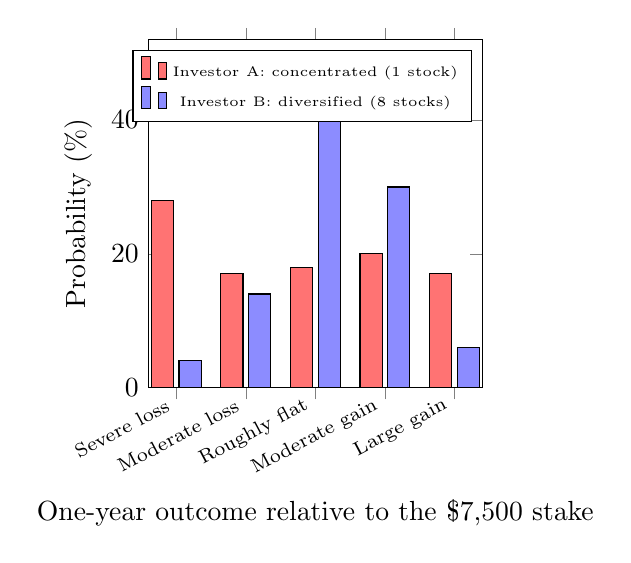
\begin{tikzpicture}
\begin{axis}[
    ybar,
    bar width=8pt,
    xlabel={One-year outcome relative to the \$7{,}500 stake},
    ylabel={Probability (\%)},
    symbolic x coords={Severe loss,Moderate loss,Roughly flat,Moderate gain,Large gain},
    xtick=data,
    x tick label style={font=\scriptsize, rotate=28, anchor=east},
    width=0.48\textwidth, height=6.0cm,
    legend pos=north east,
    legend style={font=\tiny},
    ymin=0, ymax=52
]
\addplot[fill=red!55] coordinates {(Severe loss,28)(Moderate loss,17)(Roughly flat,18)(Moderate gain,20)(Large gain,17)};
\addlegendentry{Investor A: concentrated (1 stock)}
\addplot[fill=blue!45] coordinates {(Severe loss,4)(Moderate loss,14)(Roughly flat,46)(Moderate gain,30)(Large gain,6)};
\addlegendentry{Investor B: diversified (8 stocks)}
\end{axis}
\end{tikzpicture}
\caption{Stylized illustrative one-year outcome distributions for a fixed \$7{,}500 IPO allocation, concentrated in a single name versus spread across eight names, consistent with the scenario inputs of Table~\ref{tab:scenario} and the variance-compression result of Eq.~\eqref{eq:diversification}. The diversified strategy compresses outcomes toward the moderate middle of the distribution---fewer catastrophic losses, but also a smaller chance of a single spectacular gain. Whether that trade is desirable depends on the investor's goals: for money earmarked for retirement or another essential long-run goal, compressing the loss tail at the cost of the most extreme gain tail is, for the overwhelming majority of regular investors, the financially and psychologically correct trade.}
\label{fig:wealthdist}
\end{figure}

This is the central, quantitatively provable argument of this handbook in miniature: \emph{diversification did not require Investor B to be a better stock-picker than Investor A}---it required only that Investor B split the same total bet across more names. The expected value given up (about \$408 in this illustration, on a \$50{,}000 portfolio---less than 0.1\% of total wealth) purchased a dramatic reduction in the chance of a financially painful, year-defining loss. For money that matters to an investor's long-run plan, that is very nearly always a good trade.

% ============================================================
\section{Behavioral Pitfalls and How to Pre-Commit Against Them}
\label{sec:behavioral}
% ============================================================

Even an investor who fully accepts the mathematics above can be derailed by predictable psychological forces that are, if anything, \emph{amplified} during an active IPO season:

\begin{itemize}
    \item \textbf{Fear of missing out (FOMO) and narrative bias.} Heavy media coverage of a hot listing creates a vivid, emotionally compelling story that can make a textbook ``small, diversified, rules-based allocation'' feel inadequate or even foolish in the moment---right up until the moment it is not.
    \item \textbf{Anchoring on the first-day pop.} An investor who watches a stock open 40\% above its offer price may anchor on that number as a reference point, and feel that any subsequent price below it represents a ``discount''---when, in fact, the offer price (not the opening trade) is the only price level with any documented statistical meaning, and even that meaning (Section~\ref{sec:disadvantage}) cuts against, not for, the retail buyer.
    \item \textbf{The availability heuristic and survivorship bias.} The companies a regular investor can easily recall as ``great IPOs'' are, almost by definition, the ones that succeeded spectacularly and therefore remain prominent in memory and media coverage years later---a highly non-representative sample of the full population documented in Figure~\ref{fig:longrun}.
    \item \textbf{Mental accounting.} Treating ``IPO money'' as a separate account from ``retirement money'' \cite{thaler1999} can lead an investor to take far more risk with it than they would accept for the portfolio as a whole---exactly the dynamic that the position-sizing discipline of Section~\ref{sec:strategies}.C is designed to prevent by anchoring the satellite allocation to a fixed, pre-committed percentage of \emph{total} wealth.
\end{itemize}

The standard, well-tested antidote to all four of these is \emph{pre-commitment}: deciding, in a calm moment and in writing, before the emotionally charged moment arrives, exactly what fraction of the portfolio will be devoted to IPO exposure, how it will be diversified, how it will be entered (e.g., via a DCA schedule), and under what conditions (if any) it will be trimmed or exited---and then following that plan mechanically, regardless of what the headlines say in the interim. This is precisely the function that a written \emph{investment policy statement} serves for professional fiduciaries, and there is no reason a regular investor cannot write a one-page version of their own before the first headline-grabbing listing of the season even prices.

% ============================================================
\section{A Practical Decision Checklist for the Months Ahead}
\label{sec:checklist}
% ============================================================

Drawing the preceding sections together, a regular investor facing an active IPO season can apply the following sequence of questions and rules of thumb:

\begin{enumerate}
    \item \textbf{Set the ceiling first, in writing, before any specific deal excites you.} Decide what percentage of your \emph{total investable assets}---not of ``spare cash,'' which is a mental-accounting trap---you are willing to devote to IPO exposure this season. The fractional-Kelly-with-humility calculation in Section~\ref{sec:strategies}.C suggests that, for most regular investors and for most plausible (i.e., not wildly optimistic) input assumptions, a number in the low-single-digit to low-double-digit percentage range is defensible; numbers materially above that require correspondingly more confidence in inputs that are, for any newly listed firm, genuinely very hard to estimate.
    \item \textbf{Plan to diversify across names, categories, and \emph{vintages} before you plan to pick a winner.} Section~\ref{sec:strategies}.B shows that spreading a fixed allocation across eight to twelve names removes most of the diversifiable variance at essentially no cost in expected return---a far higher-probability route to a good outcome than attempting to identify, in advance and with no track record to study, which single name will be the exception to the long-run-underperformance pattern documented in Figure~\ref{fig:longrun}.
    \item \textbf{Plan your entries before listing day, and stagger them.} Section~\ref{sec:strategies}.D shows that a staggered entry schedule mathematically guarantees an average purchase price no worse than the simple average of the prices encountered---and, just as importantly, removes the single highest-stakes, highest-emotion decision from the process.
    \item \textbf{Write down, in advance, what you will do at the lock-up date.} Section~\ref{sec:risk}.B shows that this date is public information and is associated, on average, with a predictable bout of supply-driven volatility. Knowing the date in advance converts a potential shock into an anticipated, planned-for event.
    \item \textbf{Remember that your existing index fund is already ``in the game.''} Section~\ref{sec:strategies}.E shows that a diversified core holding will, over time, organically gain exposure to whichever of this season's listings go on to matter---without requiring you to correctly identify them in advance, and without exposing you to the highest-risk earliest period of their public lives.
    \item \textbf{Re-evaluate on a fixed schedule, not in response to headlines.} Decide in advance (e.g., quarterly, alongside your regular portfolio rebalancing) when you will review the IPO sleeve's size and composition relative to your written plan---and resist the urge to make ad hoc changes in between, particularly in the days immediately following a dramatic price move in either direction.
\end{enumerate}

% ============================================================
\section{Conclusion}
\label{sec:conclusion}
% ============================================================

The months ahead are likely to bring genuine opportunity: a deep pipeline of newly public companies, some of which will, in hindsight, turn out to have been excellent long-run investments. They are also likely to bring exactly the conditions under which regular investors have historically fared worst---intense media attention, emotionally compelling narratives, a structurally tilted information and allocation landscape (Section~\ref{sec:disadvantage}), and a return distribution that is, at the level of the individual security, considerably more volatile and considerably less favorable in the long run than the first-day headlines suggest (Section~\ref{sec:risk}).

None of the tools assembled in this paper require an investor to be a better stock-picker, a faster trader, or a more sophisticated analyst than the institutions on the other side of the IPO bookbuilding process---which is fortunate, because, as Rock's model and the subsequent decades of evidence make clear, that is an extremely difficult contest for a regular investor to win on the institutions' home turf \cite{rock1986,ritter1991}. Instead, the tools require only arithmetic that any investor can perform with a basic spreadsheet: deciding on a sensible \emph{ceiling} for total exposure (Section~\ref{sec:strategies}.A, C), \emph{spreading} that exposure across enough names that no single disappointment is decisive (Section~\ref{sec:strategies}.B), \emph{spacing} purchases out over time to avoid concentrating risk in a single, emotionally charged moment (Section~\ref{sec:strategies}.D), and \emph{trusting} the diversified core holdings an investor (one hopes) already owns to do a meaningful share of the work automatically (Section~\ref{sec:strategies}.E). The worked case study in Section~\ref{sec:case} shows, with fully specified numbers, that this discipline costs an investor very little in expected return while removing a large share of the risk of a genuinely bad, plan-derailing year.

The single sentence that best summarizes the entire handbook is one that a regular investor can write on a sticky note and place on their monitor before the first headline-grabbing IPO of the season prices: \emph{the size of the bet, not the cleverness of the pick, is what determines whether an exciting opportunity becomes a wealth-building event or a wealth-destroying one---and the size of the bet is the one variable that is entirely, mathematically, within the investor's own control.}

\begin{thebibliography}{20}

\bibitem{ritter1991}
J. R. Ritter,
``The long-run performance of initial public offerings,''
\textit{The Journal of Finance}, vol. 46, no. 1, pp. 3--27, 1991.

\bibitem{loughranritter1995}
T. Loughran and J. R. Ritter,
``The new issues puzzle,''
\textit{The Journal of Finance}, vol. 50, no. 1, pp. 23--51, 1995.

\bibitem{ibbotson1975}
R. G. Ibbotson,
``Price performance of common stock new issues,''
\textit{Journal of Financial Economics}, vol. 2, no. 3, pp. 235--272, 1975.

\bibitem{rock1986}
K. Rock,
``Why new issues are underpriced,''
\textit{Journal of Financial Economics}, vol. 15, no. 1--2, pp. 187--212, 1986.

\bibitem{loughranritter2004}
T. Loughran and J. R. Ritter,
``Why has IPO underpricing changed over time?''
\textit{Financial Management}, vol. 33, no. 3, pp. 5--37, 2004.

\bibitem{lucasmcdonald1990}
D. J. Lucas and R. L. McDonald,
``Equity issues and stock price dynamics,''
\textit{The Journal of Finance}, vol. 45, no. 4, pp. 1019--1043, 1990.

\bibitem{markowitz1952}
H. Markowitz,
``Portfolio selection,''
\textit{The Journal of Finance}, vol. 7, no. 1, pp. 77--91, 1952.

\bibitem{sharpe1964}
W. F. Sharpe,
``Capital asset prices: A theory of market equilibrium under conditions of risk,''
\textit{The Journal of Finance}, vol. 19, no. 3, pp. 425--442, 1964.

\bibitem{famafrench1993}
E. F. Fama and K. R. French,
``Common risk factors in the returns on stocks and bonds,''
\textit{Journal of Financial Economics}, vol. 33, no. 1, pp. 3--56, 1993.

\bibitem{kelly1956}
J. L. Kelly Jr.,
``A new interpretation of information rate,''
\textit{Bell System Technical Journal}, vol. 35, no. 4, pp. 917--926, 1956.

\bibitem{blackscholes1973}
F. Black and M. Scholes,
``The pricing of options and corporate liabilities,''
\textit{Journal of Political Economy}, vol. 81, no. 3, pp. 637--654, 1973.

\bibitem{barberodean2000}
B. M. Barber and T. Odean,
``Trading is hazardous to your wealth: The common stock investment performance of individual investors,''
\textit{The Journal of Finance}, vol. 55, no. 2, pp. 773--806, 2000.

\bibitem{benartzithaler2001}
S. Benartzi and R. H. Thaler,
``Naive diversification strategies in defined contribution saving plans,''
\textit{American Economic Review}, vol. 91, no. 1, pp. 79--98, 2001.

\bibitem{thaler1999}
R. H. Thaler,
``Mental accounting matters,''
\textit{Journal of Behavioral Decision Making}, vol. 12, no. 3, pp. 183--206, 1999.

\bibitem{bodiekanemarcus}
Z. Bodie, A. Kane, and A. J. Marcus,
\textit{Investments}, 12th ed. New York, NY, USA: McGraw-Hill Education, 2021.

\end{thebibliography}

\end{document}
</content>
